\documentclass[twoside]{book}

% Packages required by doxygen
\usepackage{fixltx2e}
\usepackage{calc}
\usepackage{doxygen}
\usepackage[export]{adjustbox} % also loads graphicx
\usepackage{graphicx}
\usepackage[utf8]{inputenc}
\usepackage{makeidx}
\usepackage{multicol}
\usepackage{multirow}
\PassOptionsToPackage{warn}{textcomp}
\usepackage{textcomp}
\usepackage[nointegrals]{wasysym}
\usepackage[table]{xcolor}

% Font selection
\usepackage[T1]{fontenc}
\usepackage[scaled=.90]{helvet}
\usepackage{courier}
\usepackage{amssymb}
\usepackage{sectsty}
\renewcommand{\familydefault}{\sfdefault}
\allsectionsfont{%
  \fontseries{bc}\selectfont%
  \color{darkgray}%
}
\renewcommand{\DoxyLabelFont}{%
  \fontseries{bc}\selectfont%
  \color{darkgray}%
}
\newcommand{\+}{\discretionary{\mbox{\scriptsize$\hookleftarrow$}}{}{}}

% Page & text layout
\usepackage{geometry}
\geometry{%
  a4paper,%
  top=2.5cm,%
  bottom=2.5cm,%
  left=2.5cm,%
  right=2.5cm%
}
\tolerance=750
\hfuzz=15pt
\hbadness=750
\setlength{\emergencystretch}{15pt}
\setlength{\parindent}{0cm}
\setlength{\parskip}{3ex plus 2ex minus 2ex}
\makeatletter
\renewcommand{\paragraph}{%
  \@startsection{paragraph}{4}{0ex}{-1.0ex}{1.0ex}{%
    \normalfont\normalsize\bfseries\SS@parafont%
  }%
}
\renewcommand{\subparagraph}{%
  \@startsection{subparagraph}{5}{0ex}{-1.0ex}{1.0ex}{%
    \normalfont\normalsize\bfseries\SS@subparafont%
  }%
}
\makeatother

% Headers & footers
\usepackage{fancyhdr}
\pagestyle{fancyplain}
\fancyhead[LE]{\fancyplain{}{\bfseries\thepage}}
\fancyhead[CE]{\fancyplain{}{}}
\fancyhead[RE]{\fancyplain{}{\bfseries\leftmark}}
\fancyhead[LO]{\fancyplain{}{\bfseries\rightmark}}
\fancyhead[CO]{\fancyplain{}{}}
\fancyhead[RO]{\fancyplain{}{\bfseries\thepage}}
\fancyfoot[LE]{\fancyplain{}{}}
\fancyfoot[CE]{\fancyplain{}{}}
\fancyfoot[RE]{\fancyplain{}{\bfseries\scriptsize Generated by Doxygen }}
\fancyfoot[LO]{\fancyplain{}{\bfseries\scriptsize Generated by Doxygen }}
\fancyfoot[CO]{\fancyplain{}{}}
\fancyfoot[RO]{\fancyplain{}{}}
\renewcommand{\footrulewidth}{0.4pt}
\renewcommand{\chaptermark}[1]{%
  \markboth{#1}{}%
}
\renewcommand{\sectionmark}[1]{%
  \markright{\thesection\ #1}%
}

% Indices & bibliography
\usepackage{natbib}
\usepackage[titles]{tocloft}
\setcounter{tocdepth}{3}
\setcounter{secnumdepth}{5}
\makeindex

% Hyperlinks (required, but should be loaded last)
\usepackage{ifpdf}
\ifpdf
  \usepackage[pdftex,pagebackref=true]{hyperref}
\else
  \usepackage[ps2pdf,pagebackref=true]{hyperref}
\fi
\hypersetup{%
  colorlinks=true,%
  linkcolor=blue,%
  citecolor=blue,%
  unicode%
}

% Custom commands
\newcommand{\clearemptydoublepage}{%
  \newpage{\pagestyle{empty}\cleardoublepage}%
}

\usepackage{caption}
\captionsetup{labelsep=space,justification=centering,font={bf},singlelinecheck=off,skip=4pt,position=top}

%===== C O N T E N T S =====

\begin{document}

% Titlepage & ToC
\hypersetup{pageanchor=false,
             bookmarksnumbered=true,
             pdfencoding=unicode
            }
\pagenumbering{alph}
\begin{titlepage}
\vspace*{7cm}
\begin{center}%
{\Large Assignment 2 }\\
\vspace*{1cm}
{\large Generated by Doxygen 1.8.14}\\
\end{center}
\end{titlepage}
\clearemptydoublepage
\pagenumbering{roman}
\tableofcontents
\clearemptydoublepage
\pagenumbering{arabic}
\hypersetup{pageanchor=true}

%--- Begin generated contents ---
\chapter{Hierarchical Index}
\section{Class Hierarchy}
This inheritance list is sorted roughly, but not completely, alphabetically\+:\begin{DoxyCompactList}
\item \contentsline{section}{A\+A\+Lst.\+A\+A\+Lst}{\pageref{class_a_a_lst_1_1_a_a_lst}}{}
\item \contentsline{section}{D\+Cap\+A\+Lst.\+D\+Cap\+A\+Lst}{\pageref{class_d_cap_a_lst_1_1_d_cap_a_lst}}{}
\item \contentsline{section}{Read.\+Read}{\pageref{class_read_1_1_read}}{}
\item \contentsline{section}{S\+A\+Lst.\+S\+A\+Lst}{\pageref{class_s_a_lst_1_1_s_a_lst}}{}
\item \contentsline{section}{Seq\+A\+D\+T.\+Seq\+A\+DT}{\pageref{class_seq_a_d_t_1_1_seq_a_d_t}}{}
\item Enum\begin{DoxyCompactList}
\item \contentsline{section}{Stdnt\+Alloc\+Types.\+DeptT}{\pageref{class_stdnt_alloc_types_1_1_dept_t}}{}
\item \contentsline{section}{Stdnt\+Alloc\+Types.\+GenT}{\pageref{class_stdnt_alloc_types_1_1_gen_t}}{}
\end{DoxyCompactList}
\item Named\+Tuple\begin{DoxyCompactList}
\item \contentsline{section}{Stdnt\+Alloc\+Types.\+S\+InfoT}{\pageref{class_stdnt_alloc_types_1_1_s_info_t}}{}
\end{DoxyCompactList}
\end{DoxyCompactList}

\chapter{Class Index}
\section{Class List}
Here are the classes, structs, unions and interfaces with brief descriptions\+:\begin{DoxyCompactList}
\item\contentsline{section}{\mbox{\hyperlink{class_a_a_lst_1_1_a_a_lst}{A\+A\+Lst.\+A\+A\+Lst}} \\*An abstract object \mbox{\hyperlink{class_a_a_lst_1_1_a_a_lst}{A\+A\+Lst}} that contains a set of tuples (Department, str) and methods on them }{\pageref{class_a_a_lst_1_1_a_a_lst}}{}
\item\contentsline{section}{\mbox{\hyperlink{class_d_cap_a_lst_1_1_d_cap_a_lst}{D\+Cap\+A\+Lst.\+D\+Cap\+A\+Lst}} \\*A class called \mbox{\hyperlink{class_d_cap_a_lst_1_1_d_cap_a_lst}{D\+Cap\+A\+Lst}} that consists of a set of (Departments, capacity) tuples }{\pageref{class_d_cap_a_lst_1_1_d_cap_a_lst}}{}
\item\contentsline{section}{\mbox{\hyperlink{class_stdnt_alloc_types_1_1_dept_t}{Stdnt\+Alloc\+Types.\+DeptT}} \\*Creates an enumeration covering all possible departments }{\pageref{class_stdnt_alloc_types_1_1_dept_t}}{}
\item\contentsline{section}{\mbox{\hyperlink{class_stdnt_alloc_types_1_1_gen_t}{Stdnt\+Alloc\+Types.\+GenT}} \\*Creates an enumeration covering gender }{\pageref{class_stdnt_alloc_types_1_1_gen_t}}{}
\item\contentsline{section}{\mbox{\hyperlink{class_read_1_1_read}{Read.\+Read}} \\*An abstract object that handles file I/O and uses two methods }{\pageref{class_read_1_1_read}}{}
\item\contentsline{section}{\mbox{\hyperlink{class_s_a_lst_1_1_s_a_lst}{S\+A\+Lst.\+S\+A\+Lst}} \\*A class containing a list of (\textquotesingle{}macid\textquotesingle{}, S\+InfoT) tuples, and methods to add, delete and recieve information on }{\pageref{class_s_a_lst_1_1_s_a_lst}}{}
\item\contentsline{section}{\mbox{\hyperlink{class_seq_a_d_t_1_1_seq_a_d_t}{Seq\+A\+D\+T.\+Seq\+A\+DT}} \\*Creates an abstract data type that creates a sequence and provides methods to access sequence }{\pageref{class_seq_a_d_t_1_1_seq_a_d_t}}{}
\item\contentsline{section}{\mbox{\hyperlink{class_stdnt_alloc_types_1_1_s_info_t}{Stdnt\+Alloc\+Types.\+S\+InfoT}} \\*Creates a Named\+Tuple called \mbox{\hyperlink{class_stdnt_alloc_types_1_1_s_info_t}{S\+InfoT}} , containing fields and their types }{\pageref{class_stdnt_alloc_types_1_1_s_info_t}}{}
\end{DoxyCompactList}

\chapter{File Index}
\section{File List}
Here is a list of all documented files with brief descriptions\+:\begin{DoxyCompactList}
\item\contentsline{section}{\mbox{\hyperlink{_a_a_lst_8py}{A\+A\+Lst.\+py}} \\*A\+A\+Lst }{\pageref{_a_a_lst_8py}}{}
\item\contentsline{section}{\mbox{\hyperlink{_d_cap_a_lst_8py}{D\+Cap\+A\+Lst.\+py}} \\*D\+Cap\+A\+Lst }{\pageref{_d_cap_a_lst_8py}}{}
\item\contentsline{section}{\mbox{\hyperlink{_read_8py}{Read.\+py}} \\*Read }{\pageref{_read_8py}}{}
\item\contentsline{section}{\mbox{\hyperlink{_s_a_lst_8py}{S\+A\+Lst.\+py}} \\*S\+A\+Lst }{\pageref{_s_a_lst_8py}}{}
\item\contentsline{section}{\mbox{\hyperlink{_seq_a_d_t_8py}{Seq\+A\+D\+T.\+py}} \\*Seq\+A\+DT }{\pageref{_seq_a_d_t_8py}}{}
\item\contentsline{section}{\mbox{\hyperlink{_stdnt_alloc_types_8py}{Stdnt\+Alloc\+Types.\+py}} \\*Stdnt\+Alloc\+Types }{\pageref{_stdnt_alloc_types_8py}}{}
\end{DoxyCompactList}

\chapter{Class Documentation}
\hypertarget{class_a_a_lst_1_1_a_a_lst}{}\section{A\+A\+Lst.\+A\+A\+Lst Class Reference}
\label{class_a_a_lst_1_1_a_a_lst}\index{A\+A\+Lst.\+A\+A\+Lst@{A\+A\+Lst.\+A\+A\+Lst}}


An abstract object \mbox{\hyperlink{class_a_a_lst_1_1_a_a_lst}{A\+A\+Lst}} that contains a set of tuples (Department, str) and methods on them.  


\subsection*{Static Public Member Functions}
\begin{DoxyCompactItemize}
\item 
\mbox{\Hypertarget{class_a_a_lst_1_1_a_a_lst_ade2ae95f7a0e7ad568b8fdcccdc18556}\label{class_a_a_lst_1_1_a_a_lst_ade2ae95f7a0e7ad568b8fdcccdc18556}} 
def \mbox{\hyperlink{class_a_a_lst_1_1_a_a_lst_ade2ae95f7a0e7ad568b8fdcccdc18556}{init}} ()
\begin{DoxyCompactList}\small\item\em A method to initialize the set, filling it with departments of type DeptT and initally empty sequence of strings. \end{DoxyCompactList}\item 
\mbox{\Hypertarget{class_a_a_lst_1_1_a_a_lst_a6cc4b320d445656b347115c3d440be45}\label{class_a_a_lst_1_1_a_a_lst_a6cc4b320d445656b347115c3d440be45}} 
def \mbox{\hyperlink{class_a_a_lst_1_1_a_a_lst_a6cc4b320d445656b347115c3d440be45}{add\+\_\+stdnt}} (dep, m)
\begin{DoxyCompactList}\small\item\em A method to add a (DeptT, str) tuple to the set. \end{DoxyCompactList}\item 
def \mbox{\hyperlink{class_a_a_lst_1_1_a_a_lst_aecd1653cb6c7db79cff37d34294a9fc2}{lst\+\_\+alloc}} (d)
\begin{DoxyCompactList}\small\item\em A method that returns current string sequence for a given department. \end{DoxyCompactList}\item 
def \mbox{\hyperlink{class_a_a_lst_1_1_a_a_lst_a7751d151fd74a6ea51e662ab9f69284a}{num\+\_\+alloc}} (d)
\begin{DoxyCompactList}\small\item\em A method to give the length of the string sequence for a given deparment. \end{DoxyCompactList}\end{DoxyCompactItemize}
\subsection*{Static Public Attributes}
\begin{DoxyCompactItemize}
\item 
\mbox{\Hypertarget{class_a_a_lst_1_1_a_a_lst_a6ae8cae10113ada2ed31a48f853147c7}\label{class_a_a_lst_1_1_a_a_lst_a6ae8cae10113ada2ed31a48f853147c7}} 
list {\bfseries s} = \mbox{[}$\,$\mbox{]}
\end{DoxyCompactItemize}


\subsection{Detailed Description}
An abstract object \mbox{\hyperlink{class_a_a_lst_1_1_a_a_lst}{A\+A\+Lst}} that contains a set of tuples (Department, str) and methods on them. 

\subsection{Member Function Documentation}
\mbox{\Hypertarget{class_a_a_lst_1_1_a_a_lst_aecd1653cb6c7db79cff37d34294a9fc2}\label{class_a_a_lst_1_1_a_a_lst_aecd1653cb6c7db79cff37d34294a9fc2}} 
\index{A\+A\+Lst\+::\+A\+A\+Lst@{A\+A\+Lst\+::\+A\+A\+Lst}!lst\+\_\+alloc@{lst\+\_\+alloc}}
\index{lst\+\_\+alloc@{lst\+\_\+alloc}!A\+A\+Lst\+::\+A\+A\+Lst@{A\+A\+Lst\+::\+A\+A\+Lst}}
\subsubsection{\texorpdfstring{lst\+\_\+alloc()}{lst\_alloc()}}
{\footnotesize\ttfamily def A\+A\+Lst.\+A\+A\+Lst.\+lst\+\_\+alloc (\begin{DoxyParamCaption}\item[{}]{d }\end{DoxyParamCaption})\hspace{0.3cm}{\ttfamily [static]}}



A method that returns current string sequence for a given department. 


\begin{DoxyParams}{Parameters}
{\em 1} & Department of type DeptT \\
\hline
\end{DoxyParams}
\begin{DoxyReturn}{Returns}
list of strings 
\end{DoxyReturn}
\mbox{\Hypertarget{class_a_a_lst_1_1_a_a_lst_a7751d151fd74a6ea51e662ab9f69284a}\label{class_a_a_lst_1_1_a_a_lst_a7751d151fd74a6ea51e662ab9f69284a}} 
\index{A\+A\+Lst\+::\+A\+A\+Lst@{A\+A\+Lst\+::\+A\+A\+Lst}!num\+\_\+alloc@{num\+\_\+alloc}}
\index{num\+\_\+alloc@{num\+\_\+alloc}!A\+A\+Lst\+::\+A\+A\+Lst@{A\+A\+Lst\+::\+A\+A\+Lst}}
\subsubsection{\texorpdfstring{num\+\_\+alloc()}{num\_alloc()}}
{\footnotesize\ttfamily def A\+A\+Lst.\+A\+A\+Lst.\+num\+\_\+alloc (\begin{DoxyParamCaption}\item[{}]{d }\end{DoxyParamCaption})\hspace{0.3cm}{\ttfamily [static]}}



A method to give the length of the string sequence for a given deparment. 


\begin{DoxyParams}{Parameters}
{\em 1} & Department of type DeptT \\
\hline
\end{DoxyParams}
\begin{DoxyReturn}{Returns}
Int of length of string sequence 
\end{DoxyReturn}


The documentation for this class was generated from the following file\+:\begin{DoxyCompactItemize}
\item 
\mbox{\hyperlink{_a_a_lst_8py}{A\+A\+Lst.\+py}}\end{DoxyCompactItemize}

\hypertarget{class_d_cap_a_lst_1_1_d_cap_a_lst}{}\section{D\+Cap\+A\+Lst.\+D\+Cap\+A\+Lst Class Reference}
\label{class_d_cap_a_lst_1_1_d_cap_a_lst}\index{D\+Cap\+A\+Lst.\+D\+Cap\+A\+Lst@{D\+Cap\+A\+Lst.\+D\+Cap\+A\+Lst}}


A class called \mbox{\hyperlink{class_d_cap_a_lst_1_1_d_cap_a_lst}{D\+Cap\+A\+Lst}} that consists of a set of (Departments, capacity) tuples.  


\subsection*{Static Public Attributes}
\begin{DoxyCompactItemize}
\item 
\mbox{\Hypertarget{class_d_cap_a_lst_1_1_d_cap_a_lst_a3beaf12440f69c7c35f12c8fde66e139}\label{class_d_cap_a_lst_1_1_d_cap_a_lst_a3beaf12440f69c7c35f12c8fde66e139}} 
{\bfseries s} = set()
\end{DoxyCompactItemize}


\subsection{Detailed Description}
A class called \mbox{\hyperlink{class_d_cap_a_lst_1_1_d_cap_a_lst}{D\+Cap\+A\+Lst}} that consists of a set of (Departments, capacity) tuples. 

Contains methods for adding, removing, and getting tuple and department 

The documentation for this class was generated from the following file\+:\begin{DoxyCompactItemize}
\item 
\mbox{\hyperlink{_d_cap_a_lst_8py}{D\+Cap\+A\+Lst.\+py}}\end{DoxyCompactItemize}

\hypertarget{class_stdnt_alloc_types_1_1_dept_t}{}\section{Stdnt\+Alloc\+Types.\+DeptT Class Reference}
\label{class_stdnt_alloc_types_1_1_dept_t}\index{Stdnt\+Alloc\+Types.\+DeptT@{Stdnt\+Alloc\+Types.\+DeptT}}


Creates an enumeration covering all possible departments.  


Inheritance diagram for Stdnt\+Alloc\+Types.\+DeptT\+:\begin{figure}[H]
\begin{center}
\leavevmode
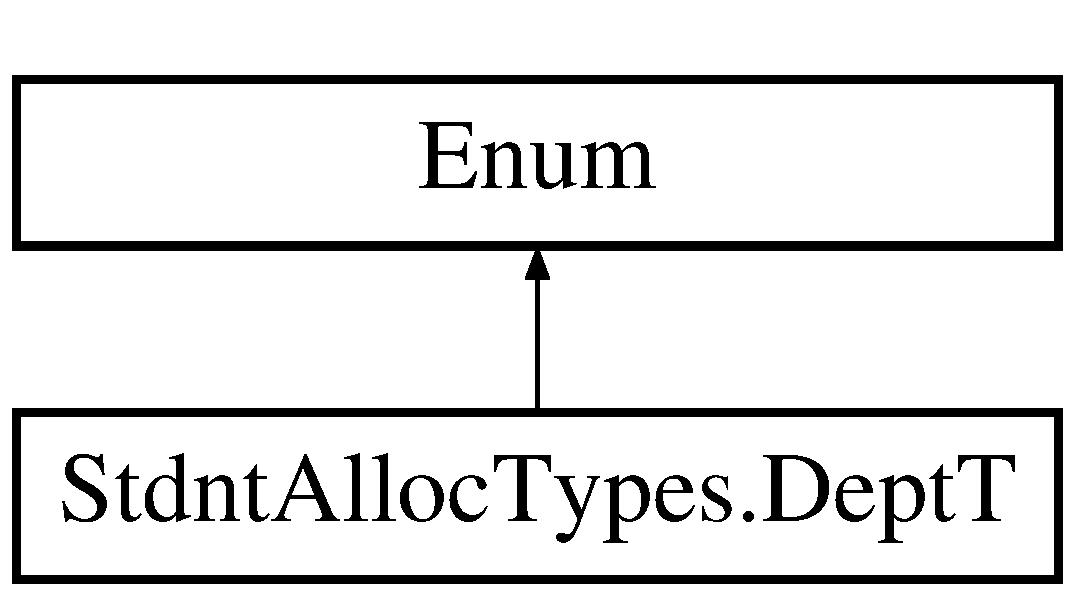
\includegraphics[height=2.000000cm]{class_stdnt_alloc_types_1_1_dept_t}
\end{center}
\end{figure}
\subsection*{Static Public Attributes}
\begin{DoxyCompactItemize}
\item 
\mbox{\Hypertarget{class_stdnt_alloc_types_1_1_dept_t_aada6de6cfa9e35835c94897913588edd}\label{class_stdnt_alloc_types_1_1_dept_t_aada6de6cfa9e35835c94897913588edd}} 
int {\bfseries civil} = 1
\item 
\mbox{\Hypertarget{class_stdnt_alloc_types_1_1_dept_t_a80264399591475d30e2b11edc8d3ed90}\label{class_stdnt_alloc_types_1_1_dept_t_a80264399591475d30e2b11edc8d3ed90}} 
int {\bfseries chemical} = 2
\item 
\mbox{\Hypertarget{class_stdnt_alloc_types_1_1_dept_t_a05ec081635b490c6c2bd52b1a236d1db}\label{class_stdnt_alloc_types_1_1_dept_t_a05ec081635b490c6c2bd52b1a236d1db}} 
int {\bfseries electrical} = 3
\item 
\mbox{\Hypertarget{class_stdnt_alloc_types_1_1_dept_t_a1aa44583eb22b8d664787fc5e82c5043}\label{class_stdnt_alloc_types_1_1_dept_t_a1aa44583eb22b8d664787fc5e82c5043}} 
int {\bfseries mechanical} = 4
\item 
\mbox{\Hypertarget{class_stdnt_alloc_types_1_1_dept_t_a1b548d82705fc0b22d69d3628aaf4e4a}\label{class_stdnt_alloc_types_1_1_dept_t_a1b548d82705fc0b22d69d3628aaf4e4a}} 
int {\bfseries software} = 5
\item 
\mbox{\Hypertarget{class_stdnt_alloc_types_1_1_dept_t_a89d19f797874a4f94621203c4a7b66e5}\label{class_stdnt_alloc_types_1_1_dept_t_a89d19f797874a4f94621203c4a7b66e5}} 
int {\bfseries materials} = 6
\item 
\mbox{\Hypertarget{class_stdnt_alloc_types_1_1_dept_t_af667a50955375f70988312c529ba7964}\label{class_stdnt_alloc_types_1_1_dept_t_af667a50955375f70988312c529ba7964}} 
int {\bfseries engphys} = 7
\end{DoxyCompactItemize}


\subsection{Detailed Description}
Creates an enumeration covering all possible departments. 

The documentation for this class was generated from the following file\+:\begin{DoxyCompactItemize}
\item 
\mbox{\hyperlink{_stdnt_alloc_types_8py}{Stdnt\+Alloc\+Types.\+py}}\end{DoxyCompactItemize}

\hypertarget{class_stdnt_alloc_types_1_1_gen_t}{}\section{Stdnt\+Alloc\+Types.\+GenT Class Reference}
\label{class_stdnt_alloc_types_1_1_gen_t}\index{Stdnt\+Alloc\+Types.\+GenT@{Stdnt\+Alloc\+Types.\+GenT}}


Creates an enumeration covering gender.  


Inheritance diagram for Stdnt\+Alloc\+Types.\+GenT\+:\begin{figure}[H]
\begin{center}
\leavevmode
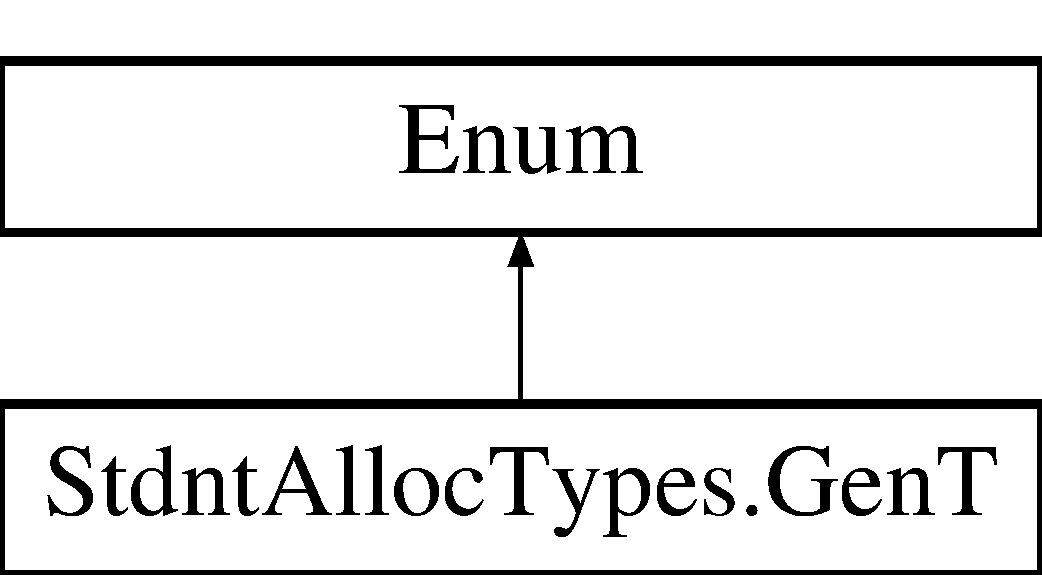
\includegraphics[height=2.000000cm]{class_stdnt_alloc_types_1_1_gen_t}
\end{center}
\end{figure}
\subsection*{Static Public Attributes}
\begin{DoxyCompactItemize}
\item 
\mbox{\Hypertarget{class_stdnt_alloc_types_1_1_gen_t_a5b77316ca7d9bd45536ba8aee60c38ca}\label{class_stdnt_alloc_types_1_1_gen_t_a5b77316ca7d9bd45536ba8aee60c38ca}} 
int {\bfseries male} = 1
\item 
\mbox{\Hypertarget{class_stdnt_alloc_types_1_1_gen_t_a5a66e845b4cfb687f41c243be4917664}\label{class_stdnt_alloc_types_1_1_gen_t_a5a66e845b4cfb687f41c243be4917664}} 
int {\bfseries female} = 2
\end{DoxyCompactItemize}


\subsection{Detailed Description}
Creates an enumeration covering gender. 



The documentation for this class was generated from the following file\+:\begin{DoxyCompactItemize}
\item 
\mbox{\hyperlink{_stdnt_alloc_types_8py}{Stdnt\+Alloc\+Types.\+py}}\end{DoxyCompactItemize}

\hypertarget{class_read_1_1_read}{}\section{Read.\+Read Class Reference}
\label{class_read_1_1_read}\index{Read.\+Read@{Read.\+Read}}


An abstract object that handles file I/O and uses two methods.  


\subsection*{Static Public Member Functions}
\begin{DoxyCompactItemize}
\item 
def \mbox{\hyperlink{class_read_1_1_read_a36ee1b801e071f6095084eb68031f4bf}{load\+\_\+stdnt\+\_\+data}} (s)
\begin{DoxyCompactList}\small\item\em A method to take in a text file, read the student information inside, and load it into S\+A\+Lst. \end{DoxyCompactList}\item 
def \mbox{\hyperlink{class_read_1_1_read_ae485f030b6a773958fdf92845df93c31}{load\+\_\+dcap\+\_\+data}} (s)
\begin{DoxyCompactList}\small\item\em A method to read a text file containing department information in the assignment, and load it into D\+Cap\+A\+Lst. \end{DoxyCompactList}\end{DoxyCompactItemize}


\subsection{Detailed Description}
An abstract object that handles file I/O and uses two methods. 

One is to read student information and load it into S\+A\+Lst. The other one is to read Deparment information and load it into D\+Cap\+A\+Lst 

\subsection{Member Function Documentation}
\mbox{\Hypertarget{class_read_1_1_read_ae485f030b6a773958fdf92845df93c31}\label{class_read_1_1_read_ae485f030b6a773958fdf92845df93c31}} 
\index{Read\+::\+Read@{Read\+::\+Read}!load\+\_\+dcap\+\_\+data@{load\+\_\+dcap\+\_\+data}}
\index{load\+\_\+dcap\+\_\+data@{load\+\_\+dcap\+\_\+data}!Read\+::\+Read@{Read\+::\+Read}}
\subsubsection{\texorpdfstring{load\+\_\+dcap\+\_\+data()}{load\_dcap\_data()}}
{\footnotesize\ttfamily def Read.\+Read.\+load\+\_\+dcap\+\_\+data (\begin{DoxyParamCaption}\item[{}]{s }\end{DoxyParamCaption})\hspace{0.3cm}{\ttfamily [static]}}



A method to read a text file containing department information in the assignment, and load it into D\+Cap\+A\+Lst. 

Each line in the file is read using list comprehension. Then, (DeptT, N) tuples are created where DeptT is the deparment and N is the capacity. Inputs them into D\+Cap\+A\+Lst 
\begin{DoxyParams}{Parameters}
{\em 1} & A string corresponding to the name of the input file \\
\hline
\end{DoxyParams}
\mbox{\Hypertarget{class_read_1_1_read_a36ee1b801e071f6095084eb68031f4bf}\label{class_read_1_1_read_a36ee1b801e071f6095084eb68031f4bf}} 
\index{Read\+::\+Read@{Read\+::\+Read}!load\+\_\+stdnt\+\_\+data@{load\+\_\+stdnt\+\_\+data}}
\index{load\+\_\+stdnt\+\_\+data@{load\+\_\+stdnt\+\_\+data}!Read\+::\+Read@{Read\+::\+Read}}
\subsubsection{\texorpdfstring{load\+\_\+stdnt\+\_\+data()}{load\_stdnt\_data()}}
{\footnotesize\ttfamily def Read.\+Read.\+load\+\_\+stdnt\+\_\+data (\begin{DoxyParamCaption}\item[{}]{s }\end{DoxyParamCaption})\hspace{0.3cm}{\ttfamily [static]}}



A method to take in a text file, read the student information inside, and load it into S\+A\+Lst. 

Takes in a text file s in the format specified. Splits each line using list comprehension and uses it to create (macid, S\+InfoT) tuples. Then add them to S\+A\+Lst 
\begin{DoxyParams}{Parameters}
{\em 1} & the name of the text file with student info \\
\hline
\end{DoxyParams}


The documentation for this class was generated from the following file\+:\begin{DoxyCompactItemize}
\item 
\mbox{\hyperlink{_read_8py}{Read.\+py}}\end{DoxyCompactItemize}

\hypertarget{class_s_a_lst_1_1_s_a_lst}{}\section{S\+A\+Lst.\+S\+A\+Lst Class Reference}
\label{class_s_a_lst_1_1_s_a_lst}\index{S\+A\+Lst.\+S\+A\+Lst@{S\+A\+Lst.\+S\+A\+Lst}}


A class containing a list of (\textquotesingle{}macid\textquotesingle{}, S\+InfoT) tuples, and methods to add, delete and recieve information on.  


\subsection*{Static Public Member Functions}
\begin{DoxyCompactItemize}
\item 
\mbox{\Hypertarget{class_s_a_lst_1_1_s_a_lst_ac0886d79feebf875207b927b6d23a959}\label{class_s_a_lst_1_1_s_a_lst_ac0886d79feebf875207b927b6d23a959}} 
def \mbox{\hyperlink{class_s_a_lst_1_1_s_a_lst_ac0886d79feebf875207b927b6d23a959}{init}} ()
\begin{DoxyCompactList}\small\item\em A method to initalize the list. \end{DoxyCompactList}\item 
def \mbox{\hyperlink{class_s_a_lst_1_1_s_a_lst_aa09d412a6f5562e32730d4857f7569ca}{add\+\_\+stdnt}} (m, i)
\begin{DoxyCompactList}\small\item\em A method to add an (m, i) tuple to the list. \end{DoxyCompactList}\item 
def \mbox{\hyperlink{class_s_a_lst_1_1_s_a_lst_a21390f23944739da71c78b8f684c7484}{remove}} (m)
\begin{DoxyCompactList}\small\item\em A method to remove a (m, i) tuple corresponding to a macid m. \end{DoxyCompactList}\item 
def \mbox{\hyperlink{class_s_a_lst_1_1_s_a_lst_ac2dc6bf81574e9e0e4a92be790460765}{elm}} (m)
\begin{DoxyCompactList}\small\item\em A method to check whether or not a (m, i) tuple corresponding to input m is in the list. \end{DoxyCompactList}\item 
def \mbox{\hyperlink{class_s_a_lst_1_1_s_a_lst_ad28fcb7dd27999a47ab1d074e69dfaa9}{info}} (m)
\begin{DoxyCompactList}\small\item\em A method to return student info give a macid. \end{DoxyCompactList}\item 
def \mbox{\hyperlink{class_s_a_lst_1_1_s_a_lst_af39c6101199578aefb42a15719754a61}{sort}} (f)
\begin{DoxyCompactList}\small\item\em a method to sort the list by a generic lambda expression \end{DoxyCompactList}\item 
\mbox{\Hypertarget{class_s_a_lst_1_1_s_a_lst_aab0e944f9f796051c78b385df084f051}\label{class_s_a_lst_1_1_s_a_lst_aab0e944f9f796051c78b385df084f051}} 
def {\bfseries getS} ()
\item 
def \mbox{\hyperlink{class_s_a_lst_1_1_s_a_lst_ae9c71d13a081d2eca72857c21840dd4b}{average}} (f)
\begin{DoxyCompactList}\small\item\em A method to calculate the average gpa of the list filtered by generic lambda method. \end{DoxyCompactList}\item 
def \mbox{\hyperlink{class_s_a_lst_1_1_s_a_lst_a8cdba5b89e936165b3628f52d4e80938}{allocate}} ()
\begin{DoxyCompactList}\small\item\em A method to allocate the students into their preferred programs. \end{DoxyCompactList}\end{DoxyCompactItemize}
\subsection*{Static Public Attributes}
\begin{DoxyCompactItemize}
\item 
\mbox{\Hypertarget{class_s_a_lst_1_1_s_a_lst_a6f08c6ea97883ece00584929a0f4db65}\label{class_s_a_lst_1_1_s_a_lst_a6f08c6ea97883ece00584929a0f4db65}} 
list {\bfseries s} = \mbox{[}$\,$\mbox{]}
\end{DoxyCompactItemize}


\subsection{Detailed Description}
A class containing a list of (\textquotesingle{}macid\textquotesingle{}, S\+InfoT) tuples, and methods to add, delete and recieve information on. 

Also contains methods to recieve average and sort by generic lambda functions, and method to allocate students 

\subsection{Member Function Documentation}
\mbox{\Hypertarget{class_s_a_lst_1_1_s_a_lst_aa09d412a6f5562e32730d4857f7569ca}\label{class_s_a_lst_1_1_s_a_lst_aa09d412a6f5562e32730d4857f7569ca}} 
\index{S\+A\+Lst\+::\+S\+A\+Lst@{S\+A\+Lst\+::\+S\+A\+Lst}!add\+\_\+stdnt@{add\+\_\+stdnt}}
\index{add\+\_\+stdnt@{add\+\_\+stdnt}!S\+A\+Lst\+::\+S\+A\+Lst@{S\+A\+Lst\+::\+S\+A\+Lst}}
\subsubsection{\texorpdfstring{add\+\_\+stdnt()}{add\_stdnt()}}
{\footnotesize\ttfamily def S\+A\+Lst.\+S\+A\+Lst.\+add\+\_\+stdnt (\begin{DoxyParamCaption}\item[{}]{m,  }\item[{}]{i }\end{DoxyParamCaption})\hspace{0.3cm}{\ttfamily [static]}}



A method to add an (m, i) tuple to the list. 

First checks the list to see if the m value is already in there if it is, raise a Key\+Error. Else, add the (m, i) tuple to the list 
\begin{DoxyParams}{Parameters}
{\em 1} & a string representing mac ids \\
\hline
{\em 2} & Student information of type S\+InfoT \\
\hline
\end{DoxyParams}
\mbox{\Hypertarget{class_s_a_lst_1_1_s_a_lst_a8cdba5b89e936165b3628f52d4e80938}\label{class_s_a_lst_1_1_s_a_lst_a8cdba5b89e936165b3628f52d4e80938}} 
\index{S\+A\+Lst\+::\+S\+A\+Lst@{S\+A\+Lst\+::\+S\+A\+Lst}!allocate@{allocate}}
\index{allocate@{allocate}!S\+A\+Lst\+::\+S\+A\+Lst@{S\+A\+Lst\+::\+S\+A\+Lst}}
\subsubsection{\texorpdfstring{allocate()}{allocate()}}
{\footnotesize\ttfamily def S\+A\+Lst.\+S\+A\+Lst.\+allocate (\begin{DoxyParamCaption}{ }\end{DoxyParamCaption})\hspace{0.3cm}{\ttfamily [static]}}



A method to allocate the students into their preferred programs. 

The method only allocates students with G\+PA 4.\+0 or higher. First, students with freechoice are sorted by G\+PA and directly placed into the programs of their choice. Next, students without free choice are allocated in based on department capacity. If students\textquotesingle{} First choice\+: if it is full, students are moved to their second choice, and so on. If a student is unable to be assigned, raise a Runtime\+Error \mbox{\Hypertarget{class_s_a_lst_1_1_s_a_lst_ae9c71d13a081d2eca72857c21840dd4b}\label{class_s_a_lst_1_1_s_a_lst_ae9c71d13a081d2eca72857c21840dd4b}} 
\index{S\+A\+Lst\+::\+S\+A\+Lst@{S\+A\+Lst\+::\+S\+A\+Lst}!average@{average}}
\index{average@{average}!S\+A\+Lst\+::\+S\+A\+Lst@{S\+A\+Lst\+::\+S\+A\+Lst}}
\subsubsection{\texorpdfstring{average()}{average()}}
{\footnotesize\ttfamily def S\+A\+Lst.\+S\+A\+Lst.\+average (\begin{DoxyParamCaption}\item[{}]{f }\end{DoxyParamCaption})\hspace{0.3cm}{\ttfamily [static]}}



A method to calculate the average gpa of the list filtered by generic lambda method. 

takes in list and filters it using lambda method. Then returns the average G\+PA. If the list is empty, raise a Value\+Error 
\begin{DoxyParams}{Parameters}
{\em 1} & generic lambda expression \\
\hline
\end{DoxyParams}
\begin{DoxyReturn}{Returns}
average of type float 
\end{DoxyReturn}
\mbox{\Hypertarget{class_s_a_lst_1_1_s_a_lst_ac2dc6bf81574e9e0e4a92be790460765}\label{class_s_a_lst_1_1_s_a_lst_ac2dc6bf81574e9e0e4a92be790460765}} 
\index{S\+A\+Lst\+::\+S\+A\+Lst@{S\+A\+Lst\+::\+S\+A\+Lst}!elm@{elm}}
\index{elm@{elm}!S\+A\+Lst\+::\+S\+A\+Lst@{S\+A\+Lst\+::\+S\+A\+Lst}}
\subsubsection{\texorpdfstring{elm()}{elm()}}
{\footnotesize\ttfamily def S\+A\+Lst.\+S\+A\+Lst.\+elm (\begin{DoxyParamCaption}\item[{}]{m }\end{DoxyParamCaption})\hspace{0.3cm}{\ttfamily [static]}}



A method to check whether or not a (m, i) tuple corresponding to input m is in the list. 


\begin{DoxyParams}{Parameters}
{\em 1} & m of type string, where \textquotesingle{}m\textquotesingle{} is a macid \\
\hline
\end{DoxyParams}
\begin{DoxyReturn}{Returns}
boolean of whether or not (m,i) is in list 
\end{DoxyReturn}
\mbox{\Hypertarget{class_s_a_lst_1_1_s_a_lst_ad28fcb7dd27999a47ab1d074e69dfaa9}\label{class_s_a_lst_1_1_s_a_lst_ad28fcb7dd27999a47ab1d074e69dfaa9}} 
\index{S\+A\+Lst\+::\+S\+A\+Lst@{S\+A\+Lst\+::\+S\+A\+Lst}!info@{info}}
\index{info@{info}!S\+A\+Lst\+::\+S\+A\+Lst@{S\+A\+Lst\+::\+S\+A\+Lst}}
\subsubsection{\texorpdfstring{info()}{info()}}
{\footnotesize\ttfamily def S\+A\+Lst.\+S\+A\+Lst.\+info (\begin{DoxyParamCaption}\item[{}]{m }\end{DoxyParamCaption})\hspace{0.3cm}{\ttfamily [static]}}



A method to return student info give a macid. 


\begin{DoxyParams}{Parameters}
{\em 1} & takes in a string pertaining to macid \\
\hline
\end{DoxyParams}
\begin{DoxyReturn}{Returns}
student information of type S\+InfotT 
\end{DoxyReturn}
\mbox{\Hypertarget{class_s_a_lst_1_1_s_a_lst_a21390f23944739da71c78b8f684c7484}\label{class_s_a_lst_1_1_s_a_lst_a21390f23944739da71c78b8f684c7484}} 
\index{S\+A\+Lst\+::\+S\+A\+Lst@{S\+A\+Lst\+::\+S\+A\+Lst}!remove@{remove}}
\index{remove@{remove}!S\+A\+Lst\+::\+S\+A\+Lst@{S\+A\+Lst\+::\+S\+A\+Lst}}
\subsubsection{\texorpdfstring{remove()}{remove()}}
{\footnotesize\ttfamily def S\+A\+Lst.\+S\+A\+Lst.\+remove (\begin{DoxyParamCaption}\item[{}]{m }\end{DoxyParamCaption})\hspace{0.3cm}{\ttfamily [static]}}



A method to remove a (m, i) tuple corresponding to a macid m. 

First check whether m is in list. If it isnt, raise Key\+Error Exception Else, remove (m, i) tuple corresponding to m 
\begin{DoxyParams}{Parameters}
{\em 1} & m of type string, corresponding to mac id \\
\hline
\end{DoxyParams}
\mbox{\Hypertarget{class_s_a_lst_1_1_s_a_lst_af39c6101199578aefb42a15719754a61}\label{class_s_a_lst_1_1_s_a_lst_af39c6101199578aefb42a15719754a61}} 
\index{S\+A\+Lst\+::\+S\+A\+Lst@{S\+A\+Lst\+::\+S\+A\+Lst}!sort@{sort}}
\index{sort@{sort}!S\+A\+Lst\+::\+S\+A\+Lst@{S\+A\+Lst\+::\+S\+A\+Lst}}
\subsubsection{\texorpdfstring{sort()}{sort()}}
{\footnotesize\ttfamily def S\+A\+Lst.\+S\+A\+Lst.\+sort (\begin{DoxyParamCaption}\item[{}]{f }\end{DoxyParamCaption})\hspace{0.3cm}{\ttfamily [static]}}



a method to sort the list by a generic lambda expression 

First, sorts the list in descending order. Next, takes in a generic lambda expression as input and uses it to filter list using filter() returns filterd list 
\begin{DoxyParams}{Parameters}
{\em 1} & lambda expression \\
\hline
\end{DoxyParams}
\begin{DoxyReturn}{Returns}
List of tuples (m, i) where m is macid of type string and i is student info of type S\+InfoT 
\end{DoxyReturn}


The documentation for this class was generated from the following file\+:\begin{DoxyCompactItemize}
\item 
\mbox{\hyperlink{_s_a_lst_8py}{S\+A\+Lst.\+py}}\end{DoxyCompactItemize}

\hypertarget{class_seq_a_d_t_1_1_seq_a_d_t}{}\section{Seq\+A\+D\+T.\+Seq\+A\+DT Class Reference}
\label{class_seq_a_d_t_1_1_seq_a_d_t}\index{Seq\+A\+D\+T.\+Seq\+A\+DT@{Seq\+A\+D\+T.\+Seq\+A\+DT}}


Creates an abstract data type that creates a sequence and provides methods to access sequence.  


\subsection*{Public Member Functions}
\begin{DoxyCompactItemize}
\item 
def \mbox{\hyperlink{class_seq_a_d_t_1_1_seq_a_d_t_a274f6f35c4d7221955ff721ab88b12e1}{\+\_\+\+\_\+init\+\_\+\+\_\+}} (self, s)
\begin{DoxyCompactList}\small\item\em Method to initialize sequence. \end{DoxyCompactList}\item 
\mbox{\Hypertarget{class_seq_a_d_t_1_1_seq_a_d_t_ad89d5ccf139e928a65000f00e605692e}\label{class_seq_a_d_t_1_1_seq_a_d_t_ad89d5ccf139e928a65000f00e605692e}} 
def \mbox{\hyperlink{class_seq_a_d_t_1_1_seq_a_d_t_ad89d5ccf139e928a65000f00e605692e}{start}} (self)
\begin{DoxyCompactList}\small\item\em Method to return sequence to start. \end{DoxyCompactList}\item 
def \mbox{\hyperlink{class_seq_a_d_t_1_1_seq_a_d_t_a1d2ee97ccd784507ae32c00150dc6fb0}{next}} (self)
\begin{DoxyCompactList}\small\item\em Method to advance to next value in sequence. \end{DoxyCompactList}\item 
def \mbox{\hyperlink{class_seq_a_d_t_1_1_seq_a_d_t_a7d8df17dae5df548ca32054075ca04b8}{end}} (self)
\begin{DoxyCompactList}\small\item\em Method to check whether we reached the end of the sequence. \end{DoxyCompactList}\end{DoxyCompactItemize}
\subsection*{Public Attributes}
\begin{DoxyCompactItemize}
\item 
\mbox{\Hypertarget{class_seq_a_d_t_1_1_seq_a_d_t_a1c751be49f197faecbd36352484be18d}\label{class_seq_a_d_t_1_1_seq_a_d_t_a1c751be49f197faecbd36352484be18d}} 
{\bfseries s}
\item 
\mbox{\Hypertarget{class_seq_a_d_t_1_1_seq_a_d_t_a9c8c61691d99a130acbfd6f4c50e3ee0}\label{class_seq_a_d_t_1_1_seq_a_d_t_a9c8c61691d99a130acbfd6f4c50e3ee0}} 
{\bfseries i}
\item 
\mbox{\Hypertarget{class_seq_a_d_t_1_1_seq_a_d_t_ad37e0e1d6faab8f674532dcbccb31384}\label{class_seq_a_d_t_1_1_seq_a_d_t_ad37e0e1d6faab8f674532dcbccb31384}} 
{\bfseries out}
\end{DoxyCompactItemize}


\subsection{Detailed Description}
Creates an abstract data type that creates a sequence and provides methods to access sequence. 



\subsection{Constructor \& Destructor Documentation}
\mbox{\Hypertarget{class_seq_a_d_t_1_1_seq_a_d_t_a274f6f35c4d7221955ff721ab88b12e1}\label{class_seq_a_d_t_1_1_seq_a_d_t_a274f6f35c4d7221955ff721ab88b12e1}} 
\index{Seq\+A\+D\+T\+::\+Seq\+A\+DT@{Seq\+A\+D\+T\+::\+Seq\+A\+DT}!\+\_\+\+\_\+init\+\_\+\+\_\+@{\+\_\+\+\_\+init\+\_\+\+\_\+}}
\index{\+\_\+\+\_\+init\+\_\+\+\_\+@{\+\_\+\+\_\+init\+\_\+\+\_\+}!Seq\+A\+D\+T\+::\+Seq\+A\+DT@{Seq\+A\+D\+T\+::\+Seq\+A\+DT}}
\subsubsection{\texorpdfstring{\+\_\+\+\_\+init\+\_\+\+\_\+()}{\_\_init\_\_()}}
{\footnotesize\ttfamily def Seq\+A\+D\+T.\+Seq\+A\+D\+T.\+\_\+\+\_\+init\+\_\+\+\_\+ (\begin{DoxyParamCaption}\item[{}]{self,  }\item[{}]{s }\end{DoxyParamCaption})}



Method to initialize sequence. 


\begin{DoxyParams}{Parameters}
{\em 1} & Takes in a list s \\
\hline
\end{DoxyParams}


\subsection{Member Function Documentation}
\mbox{\Hypertarget{class_seq_a_d_t_1_1_seq_a_d_t_a7d8df17dae5df548ca32054075ca04b8}\label{class_seq_a_d_t_1_1_seq_a_d_t_a7d8df17dae5df548ca32054075ca04b8}} 
\index{Seq\+A\+D\+T\+::\+Seq\+A\+DT@{Seq\+A\+D\+T\+::\+Seq\+A\+DT}!end@{end}}
\index{end@{end}!Seq\+A\+D\+T\+::\+Seq\+A\+DT@{Seq\+A\+D\+T\+::\+Seq\+A\+DT}}
\subsubsection{\texorpdfstring{end()}{end()}}
{\footnotesize\ttfamily def Seq\+A\+D\+T.\+Seq\+A\+D\+T.\+end (\begin{DoxyParamCaption}\item[{}]{self }\end{DoxyParamCaption})}



Method to check whether we reached the end of the sequence. 

Checks whether index is greater or equal to len(\+Seq\+A\+D\+T). If it is, we reached the end of the sequence \begin{DoxyReturn}{Returns}
boolean of whether or not we reached the end 
\end{DoxyReturn}
\mbox{\Hypertarget{class_seq_a_d_t_1_1_seq_a_d_t_a1d2ee97ccd784507ae32c00150dc6fb0}\label{class_seq_a_d_t_1_1_seq_a_d_t_a1d2ee97ccd784507ae32c00150dc6fb0}} 
\index{Seq\+A\+D\+T\+::\+Seq\+A\+DT@{Seq\+A\+D\+T\+::\+Seq\+A\+DT}!next@{next}}
\index{next@{next}!Seq\+A\+D\+T\+::\+Seq\+A\+DT@{Seq\+A\+D\+T\+::\+Seq\+A\+DT}}
\subsubsection{\texorpdfstring{next()}{next()}}
{\footnotesize\ttfamily def Seq\+A\+D\+T.\+Seq\+A\+D\+T.\+next (\begin{DoxyParamCaption}\item[{}]{self }\end{DoxyParamCaption})}



Method to advance to next value in sequence. 

Returns the current value, than moves index up by one. raises exception if we move past the end of sequence \begin{DoxyReturn}{Returns}
Returns current \mbox{\hyperlink{class_seq_a_d_t_1_1_seq_a_d_t}{Seq\+A\+DT}} value 
\end{DoxyReturn}


The documentation for this class was generated from the following file\+:\begin{DoxyCompactItemize}
\item 
\mbox{\hyperlink{_seq_a_d_t_8py}{Seq\+A\+D\+T.\+py}}\end{DoxyCompactItemize}

\hypertarget{class_stdnt_alloc_types_1_1_s_info_t}{}\section{Stdnt\+Alloc\+Types.\+S\+InfoT Class Reference}
\label{class_stdnt_alloc_types_1_1_s_info_t}\index{Stdnt\+Alloc\+Types.\+S\+InfoT@{Stdnt\+Alloc\+Types.\+S\+InfoT}}


Creates a Named\+Tuple called \mbox{\hyperlink{class_stdnt_alloc_types_1_1_s_info_t}{S\+InfoT}} , containing fields and their types.  


Inheritance diagram for Stdnt\+Alloc\+Types.\+S\+InfoT\+:\begin{figure}[H]
\begin{center}
\leavevmode
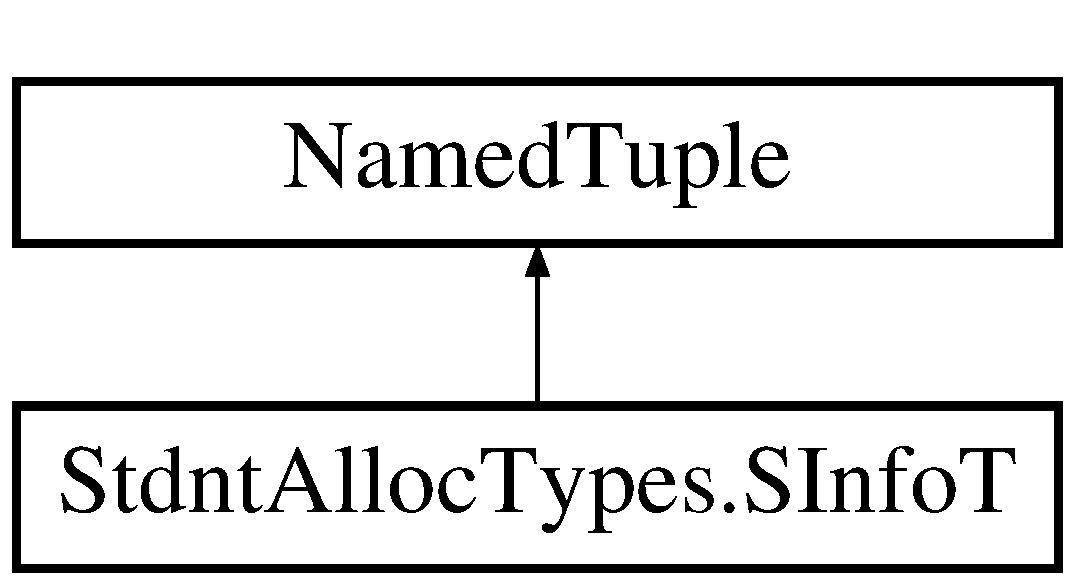
\includegraphics[height=2.000000cm]{class_stdnt_alloc_types_1_1_s_info_t}
\end{center}
\end{figure}


\subsection{Detailed Description}
Creates a Named\+Tuple called \mbox{\hyperlink{class_stdnt_alloc_types_1_1_s_info_t}{S\+InfoT}} , containing fields and their types. 

Fields are fname\+: string, lname\+: string, gender\+: \mbox{\hyperlink{class_stdnt_alloc_types_1_1_gen_t}{GenT}} enum, gpa \+: float choices\+: Seq\+A\+DT sequence A\+DT, freechoice\+: boolean 

The documentation for this class was generated from the following file\+:\begin{DoxyCompactItemize}
\item 
\mbox{\hyperlink{_stdnt_alloc_types_8py}{Stdnt\+Alloc\+Types.\+py}}\end{DoxyCompactItemize}

\chapter{File Documentation}
\hypertarget{_a_a_lst_8py}{}\section{A\+A\+Lst.\+py File Reference}
\label{_a_a_lst_8py}\index{A\+A\+Lst.\+py@{A\+A\+Lst.\+py}}


A\+A\+Lst  


\subsection*{Classes}
\begin{DoxyCompactItemize}
\item 
class \mbox{\hyperlink{class_a_a_lst_1_1_a_a_lst}{A\+A\+Lst.\+A\+A\+Lst}}
\begin{DoxyCompactList}\small\item\em An abstract object \mbox{\hyperlink{class_a_a_lst_1_1_a_a_lst}{A\+A\+Lst}} that contains a set of tuples (Department, str) and methods on them. \end{DoxyCompactList}\end{DoxyCompactItemize}


\subsection{Detailed Description}
A\+A\+Lst 

\begin{DoxyAuthor}{Author}
Jame Tran 
\end{DoxyAuthor}
\begin{DoxyDate}{Date}
Feb.\+16, 2019 
\end{DoxyDate}

\hypertarget{_d_cap_a_lst_8py}{}\section{D\+Cap\+A\+Lst.\+py File Reference}
\label{_d_cap_a_lst_8py}\index{D\+Cap\+A\+Lst.\+py@{D\+Cap\+A\+Lst.\+py}}


D\+Cap\+A\+Lst  


\subsection*{Classes}
\begin{DoxyCompactItemize}
\item 
class \mbox{\hyperlink{class_d_cap_a_lst_1_1_d_cap_a_lst}{D\+Cap\+A\+Lst.\+D\+Cap\+A\+Lst}}
\begin{DoxyCompactList}\small\item\em A class called \mbox{\hyperlink{class_d_cap_a_lst_1_1_d_cap_a_lst}{D\+Cap\+A\+Lst}} that consists of a set of (Departments, capacity) tuples. \end{DoxyCompactList}\end{DoxyCompactItemize}


\subsection{Detailed Description}
D\+Cap\+A\+Lst 

\begin{DoxyAuthor}{Author}
Jame Tran 
\end{DoxyAuthor}
\begin{DoxyDate}{Date}
Feb.\+16, 2019 
\end{DoxyDate}

\hypertarget{_read_8py}{}\section{Read.\+py File Reference}
\label{_read_8py}\index{Read.\+py@{Read.\+py}}


Read  


\subsection*{Classes}
\begin{DoxyCompactItemize}
\item 
class \mbox{\hyperlink{class_read_1_1_read}{Read.\+Read}}
\begin{DoxyCompactList}\small\item\em An abstract object that handles file I/O and uses two methods. \end{DoxyCompactList}\end{DoxyCompactItemize}


\subsection{Detailed Description}
Read 

\begin{DoxyAuthor}{Author}
Jame Tran 
\end{DoxyAuthor}
\begin{DoxyDate}{Date}
Feb.\+16, 2019 
\end{DoxyDate}

\hypertarget{_s_a_lst_8py}{}\section{S\+A\+Lst.\+py File Reference}
\label{_s_a_lst_8py}\index{S\+A\+Lst.\+py@{S\+A\+Lst.\+py}}


S\+A\+Lst  


\subsection*{Classes}
\begin{DoxyCompactItemize}
\item 
class \mbox{\hyperlink{class_s_a_lst_1_1_s_a_lst}{S\+A\+Lst.\+S\+A\+Lst}}
\begin{DoxyCompactList}\small\item\em A class containing a list of (\textquotesingle{}macid\textquotesingle{}, S\+InfoT) tuples, and methods to add, delete and recieve information on. \end{DoxyCompactList}\end{DoxyCompactItemize}


\subsection{Detailed Description}
S\+A\+Lst 

\begin{DoxyAuthor}{Author}
Jame Tran 
\end{DoxyAuthor}
\begin{DoxyDate}{Date}
Feb.\+16, 2019 
\end{DoxyDate}

\hypertarget{_seq_a_d_t_8py}{}\section{Seq\+A\+D\+T.\+py File Reference}
\label{_seq_a_d_t_8py}\index{Seq\+A\+D\+T.\+py@{Seq\+A\+D\+T.\+py}}


Seq\+A\+DT  


\subsection*{Classes}
\begin{DoxyCompactItemize}
\item 
class \mbox{\hyperlink{class_seq_a_d_t_1_1_seq_a_d_t}{Seq\+A\+D\+T.\+Seq\+A\+DT}}
\begin{DoxyCompactList}\small\item\em Creates an abstract data type that creates a sequence and provides methods to access sequence. \end{DoxyCompactList}\end{DoxyCompactItemize}


\subsection{Detailed Description}
Seq\+A\+DT 

\begin{DoxyAuthor}{Author}
Jame Tran 
\end{DoxyAuthor}
\begin{DoxyDate}{Date}
Feb.\+16, 2019 
\end{DoxyDate}

\hypertarget{_stdnt_alloc_types_8py}{}\section{Stdnt\+Alloc\+Types.\+py File Reference}
\label{_stdnt_alloc_types_8py}\index{Stdnt\+Alloc\+Types.\+py@{Stdnt\+Alloc\+Types.\+py}}


Stdnt\+Alloc\+Types  


\subsection*{Classes}
\begin{DoxyCompactItemize}
\item 
class \mbox{\hyperlink{class_stdnt_alloc_types_1_1_gen_t}{Stdnt\+Alloc\+Types.\+GenT}}
\begin{DoxyCompactList}\small\item\em Creates an enumeration covering gender. \end{DoxyCompactList}\item 
class \mbox{\hyperlink{class_stdnt_alloc_types_1_1_dept_t}{Stdnt\+Alloc\+Types.\+DeptT}}
\begin{DoxyCompactList}\small\item\em Creates an enumeration covering all possible departments. \end{DoxyCompactList}\item 
class \mbox{\hyperlink{class_stdnt_alloc_types_1_1_s_info_t}{Stdnt\+Alloc\+Types.\+S\+InfoT}}
\begin{DoxyCompactList}\small\item\em Creates a Named\+Tuple called \mbox{\hyperlink{class_stdnt_alloc_types_1_1_s_info_t}{S\+InfoT}} , containing fields and their types. \end{DoxyCompactList}\end{DoxyCompactItemize}


\subsection{Detailed Description}
Stdnt\+Alloc\+Types 

\begin{DoxyAuthor}{Author}
Jame Tran 
\end{DoxyAuthor}
\begin{DoxyDate}{Date}
Feb.\+16, 2019 
\end{DoxyDate}

%--- End generated contents ---

% Index
\backmatter
\newpage
\phantomsection
\clearemptydoublepage
\addcontentsline{toc}{chapter}{Index}
\printindex

\end{document}
